\chapter{Implementation of methods}
\label{cha:implementation_methods}

\section{Feature Selection methods} % (fold)
\label{sec:feature_selection}

\subsection{PCA - Principal Component Analysis} % (fold)
\label{sec:pca}

\begin{figure}[h]
    \centering
    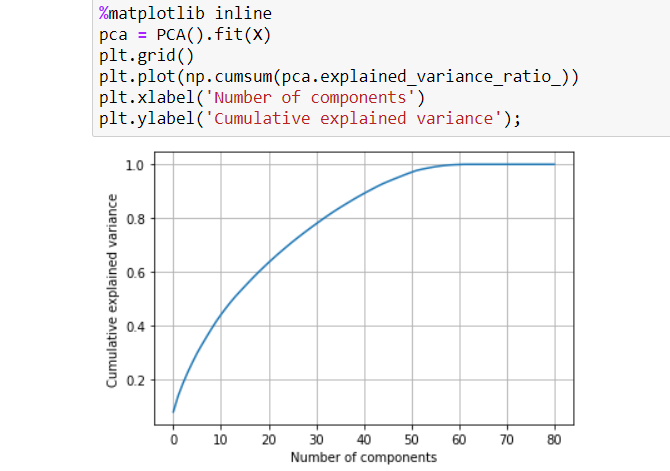
\includegraphics[width=0.75\textwidth,height=0.3\textheight]{Chapters/Figures/pca_components.png}
    \caption{Normalized X data}
    \label{fig:variance_graph}
\end{figure}


\begin{lstlisting}[language=Python]
# Calculate the variance explained by principle components
print("Variance_of_each_component:", pca.explained_variance_ratio_)
print("Total_Variance:Explained:", 
        round(sum(list(pca.explained_variance_ratio_))*100, 2))
\end{lstlisting}


\begin{figure}[h]
    \centering
    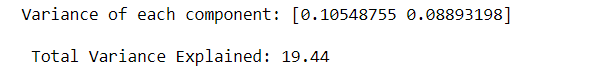
\includegraphics[width=0.6\textwidth,height=0.06\textheight]{Chapters/Figures/pca_2_comp_variance.png}
    \caption{Normalized X data}
    \label{fig:total_variance}
\end{figure}




\subsection{SOM - Self Organizing Maps} % (fold)
\label{sec:som}

\subsection{LDA - Linear Driscriminant Analysis} % (fold)
\label{sec:lda}

\section{Feature Extraction methods} % (fold)
\label{sec:feature_extraction}


\subsection{Univariate Filtering} % (fold)
\label{sec:inserting_tables}

\subsubsection{Chi-Square test} % (fold)
\label{sec:inserting_tables}

\subsubsection{ANOVA F-test} % (fold)
\label{sec:inserting_tables}

\subsection{Multivariate Filtering} % (fold)
\label{sec:inserting_tables}

\subsubsection{CFS – Correlation Based Feature Selection} % (fold)
\label{sec:inserting_tables}

\subsubsection{MRMR – Minimum Redundancy Maximum Relevance} % (fold)
\label{sec:inserting_tables}